\subsubsection{Gallery of Model Fits to Supra-threshold Experiments}

% TODO make multi panel.

\begin{figure}
    \centering
    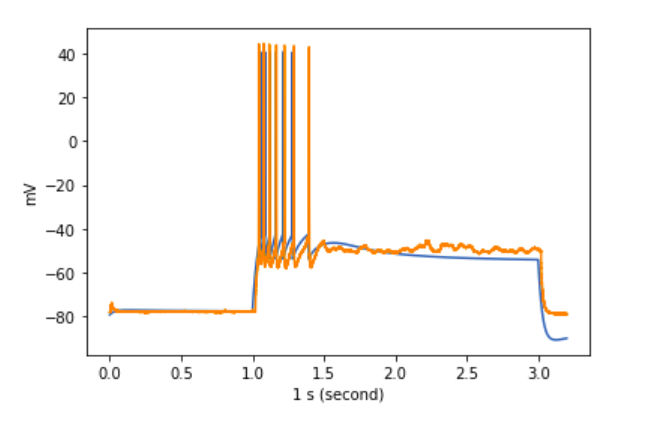
\includegraphics[scale=0.75]{figures/adexp_fit_allen_spec_id_476053392.png}
    \caption{An adaptive Exponential Model was fitted to both the spike time, and spike shape data in a sweep from Allen specimin id: 476053392} \label{fig:specimen_476053392}
\end{figure}

\begin{figure}
    \centering
    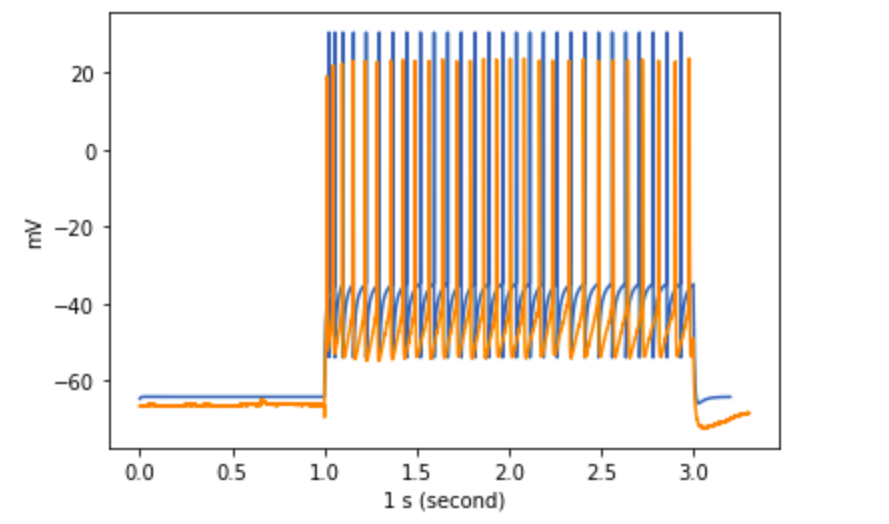
\includegraphics[scale=0.75]{figures/NU_BBP_fusion_L5PC_files/28spikesB95.png}
    \caption{An adaptive Exponential Model was fitted to both the spike time, and spike shape data in a sweep from Allen specimin id: 476053392} \label{fig:specimen_476053392}
\end{figure}

%Similar to Druckmann Suprathreshold depolarizing step currents \cite{druckmann2008evaluating}.
\begin{figure}
    \centering
    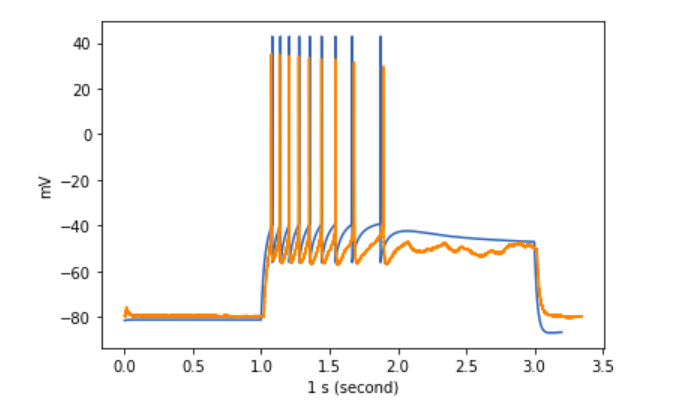
\includegraphics[scale=0.75]{figures/adexp_fit_allen_specid_325479788.png}
    \caption{ An adaptive Exponential Model was fitted to both the spike time, and spike shape data in a sweep from Allen specimin id: 325479788}
    \label{fig:specimen_325479788}
\end{figure}


% Interesting direct qoute from Druckmann:
%"In experiments, intrinsic noise gives rise to a large variability (e.g., in firing pattern) in the voltage responses to repetitions of the exact same input. Thus, the common approach of fitting models by attempting to perfectly replicate, point by point, a single chosen trace out of the spectrum of variable responses does not seem to do justice to the data."

%In experiments, however, when the exactly same stimulus is repeated several times, the voltage traces elicited differ among themselves to a significant degree (Mainen and Sejnowski, 1995; Nowak et al., 1997).

A joint collection of current injections and recordings known as sweeps were taken from a rat somato-sensory hind limb neuron.
\ref{fig:B95Adexp} is a challenging waveform to fit, as adaption does not predict the penultimate ISI, which is larger than the final one. Although it is not obvious there is relatively high CV. It is probably a bad idea to spend too much time fitting to exact spike times because neurons themselves experience noisy intrinsic currents and they are likely to illicit different spike trains, given presentation of identical stimulus.

\begin{figure}
    \centering
    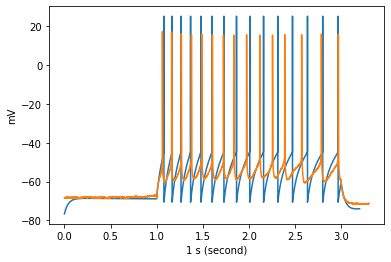
\includegraphics[scale=0.75]{figures/bbp_multispiking_fit.png}
    \caption{An adaptive Exponential Model was fitted to both the spike time, and spike shape data in a sweep from animal B95 \url{http://microcircuits.epfl.ch/#/animal/8ecde7d1-b2d2-11e4-b949-6003088da632} Blue Brain Project. The base voltage. The base voltage, and Resting Membrane Potential, and spike numbers are matched, spike times are not perfectly aligned, spike height, and trough depth are not perfectly matched}
    \label{fig:B95Adexp}
\end{figure}

\begin{figure}
    \centering
    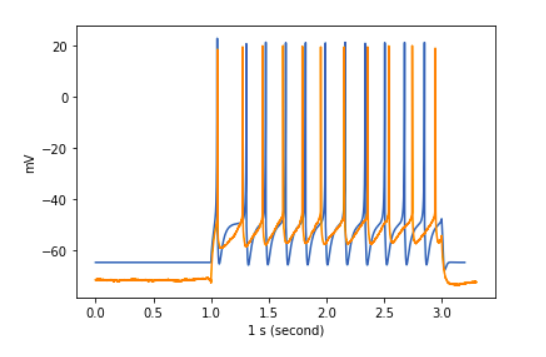
\includegraphics{figures/IZHI_B95.png}
    \caption{An Izhikevich model was fitted to both the spike time, and spike shape data in a sweep from Blue Brain Project. The Spike amplitude, and spike numbers are matched, spike times are not perfectly aligned}
    \label{fig:B95_IZHI}
\end{figure}

In figures \ref{fig:B95Adexp}, you can see that although several aspects of the waveform are fitted, exact spike times are not always fitted \ref{fig:B95_IZHI}

